%Stil på uppsats
\documentclass[11pt]{article}
\usepackage[utf8]{inputenc}
\usepackage[swedish]{babel}
\usepackage{verbatim}
\renewcommand{\baselinestretch}{1.2}
\renewcommand{\arraystretch}{0.85}

\usepackage{makecell}
\setcellgapes{5pt}

\usepackage{tabularx}
\newcolumntype{Y}{>{\centering\arraybackslash}X}

%Skippa indrag av brödtext
\usepackage{parskip}

%Bilder sida vid sida
\usepackage{subfig}

% Formattera text
\usepackage[text={12cm,20cm}]{geometry}

\usepackage{booktabs}
\usepackage{floatrow}
\floatsetup[table]{capposition=top}
\usepackage{amsmath}
\usepackage{upgreek}
\usepackage{graphicx}
\graphicspath{{./images/}}
\usepackage{textgreek}
\usepackage{sectsty}
\usepackage[autostyle]{csquotes} %citattecken 
\MakeOuterQuote{"}



\numberwithin{equation}{section}
\numberwithin{table}{section}
\numberwithin{figure}{section}

\usepackage{titlesec}
\titleformat*{\section}{\Large\bfseries}
\titleformat*{\subsection}{\large\bfseries}
\titleformat*{\subsubsection}{\small\bfseries}



\usepackage[table,xcdraw]{xcolor}

\usepackage{afterpage}
\usepackage{sectsty}
\usepackage[labelfont=bf]{caption}
\usepackage{url}
\usepackage{hyperref}
\usepackage{array}
\usepackage{multirow}

% Bibliography
\usepackage[style=authoryear,sorting=nty]{biblatex} %Imports biblatex package
\addbibresource{references.bib} %Import the bibliography file

\usepackage[referable]{threeparttablex}
\usepackage{booktabs}
\usepackage{lipsum}

\usepackage[export]{adjustbox} %För titelsida


\begin{document}



\begin{titlepage}
\thispagestyle{empty}
	\begin{figure}[ht]
	   \minipage{0.7\textwidth}
			\includegraphics[width=4cm]{su2.jpeg}
			
	   \endminipage
	    \minipage{0.6\textwidth}
		 \Large Kandidatuppsats \par
		 \large Statisiska institutionen \par
		  \small Bachelor thesis, Department of   Statistics \par
		   \large Nr 2021:1 \par
			
\endminipage
\end{figure}
	
	
\centering
\vspace{5cm}

{\large\bfseries Prognosticering av småbolagsindex: En jämförelse mellan LSTM och ARMA-GARCH\par}
	\vspace{0.5cm}

% LSTM och ARMA-GARCH: En jämförelse på ett svenskt småbolagsindex / LSTM and ARMA-GARCH: A comparison on a Swedish Small Cap index.
% Prognosticera småbolagsindex: En jämförelse mellan LSTM och ARMA-GARCH. / Predicting Small Cap index: A comparison between LSTM and ARMA-GARCH
	
{\large\itshape Predicting Small Cap index: A comparison between LSTM and ARMA-GARCH \par}
	\vfill
	
	

{\Large Erik Billebjer Ulrikson och Erik Carle\par}
	\vspace{0.5cm}
	
\begin{flushleft}
Självständigt arbete 15 högskolepoäng inom Statistik III, VT2021 \\
Handledare: Ulf Högnäs\\

\end{flushleft}
\end{titlepage}

%%%%%%%%%%%% ABSTRACT %%%%%%%%%%%%%%%%%
\newpage
\thispagestyle{empty}
\section*{Sammanfattning}
I denna studie jämförs en ekonometrisk modell, ARMA-GARCH, med en djupinlärningsmodell, LSTM, på ett svenskt småbolagsindex. Det finns en brist på studier som jämför djupinlärningsmodeller med GARCH-modeller, framförallt på svenska börsindex, vilket denna studie söker att bidra med. Studien ämnar dels att besvara om djupinlärningsmodellen med fördel kan användas istället för den ekonometriska modellen samt dels om en algoritmisk handelsstrategi som ger högre avkastning än det berörda indexet kan skapas. Modellerna korsvalideras över 1.000 skattningar och utvärderas med MAPE, RMSE, precision, känslighet, F-värde och avkastning från simulerad handel. Resultatet visar att ARMA-GARCH i genomsnitt är mer exakt och genererar högre avkastning än LSTM. Mäts prestation i prediktionsfel är modellerna dock oskiljbara. Studien visar även att ARMA-GARCH, men inte LSTM, kan användas för att skapa en algoritmisk handelsstrategi som överpresterar utvecklingen av indexet under den givna perioden. 

\newpage
\section*{Förord}
Vi vill rikta ett stort tack till vår handledare Ulf Högnäs som ställt upp på
videosamtal och gett oss konstruktiv kritik under hela processen. \bigbreak

Stockholm, maj 2021 \\
Erik \& Erik
\null
\newpage

%%%%%%%%%%%% TABLE OF CONTENTS %%%%%%%%%%%%%%%%%
\newpage
\thispagestyle{empty}
    \tableofcontents
\thispagestyle{empty}
\newpage

%%%%%%%%%%%%%% Förkortningar %%%%%%%%%%%%%%%
\newpage 
\thispagestyle{empty}

\section*{Förkortningar}
\textbf{ADF-test} \dots Augmented Dickey-Fuller-test \par
\textbf{AIC} \dots Akaike Information Criterion \par
\textbf{ANN} \dots Artifical Neural Network \par
\textbf{ARCH} \dots Autoregressive Conditional Heteroskedasticity \par
\textbf{ARIMA} \dots Autoregressive Integrated Moving Average \par
\textbf{ARMA} \dots Autoregressive Moving Average \par 
\textbf{ARMA-GARCH} \dots Autoregressive Moving Average - Generalized Autoregressive Conditional Heteroskedasticity \par 
\textbf{BIC} \dots Schwarz Bayesian Information Criterion \par
\textbf{EMH} \dots Efficient Market Hypothesis \par
\textbf{GARCH} \dots Generalized Autoregressive Conditional Heteroskedasticity \par
\textbf{LM-test} \dots Lagrange Multiplier-test \par
\textbf{LSTM} \dots Long Short-Term Memory \par
\textbf{MAPE} \dots Mean Absolute Percentage Error \par
\textbf{OMXSSC} \dots OMX Stockholm Small Cap \par
\textbf{RMSE} \dots Root-Mean-Square Error \par
\textbf{RNN} \dots Recurrent Neural Network \par


\newpage
%%%%%%%%%%%%%% INLEDNING %%%%%%%%%%%%%%%
\clearpage
\setcounter{page}{1}


\section{Inledning}
Efter att New York Stock Exchange började tillåta handel med programvara på 1980-talet populariserades algoritmisk handel.  Idag sker en stor del av all handeln på finansmarknaden automatiskt med algoritmer, år 2012 utgjorde exempelvis algoritmisk handel 85 procent av marknadsvolymen på den amerikanska börsen \parencite[][,s.258]{glantz2013multi}. Denna utveckling har i stort sin grund i den breda utecklingen av avancerad programvara och ökade möjligheter att samla in och lagra stora mängder data. Detta är en uveckling som småsparare såväl som större aktörerna såsom investmentbanker och hedgefonder dragit nytta av \parencite{DE_Shaw}. Det har publicerats ett stort antal akademiska studier som visar på att algoritmer som använder artificiella neurala nätverk, så kallade djupinlärningsmodeller, istället för ekonometriska modeller (såsom ARIMA, GARCH mfl.) med fördel kan implementeras för att generera högre avkastning än index \parencite{paliwal2009neural}. En vanligt förekommande djupinlärningsmodell är LSTM (Long Short-Term Memory) som är en typ av neuralt nätverk med egenskapen att lära sig långsiktiga mönster i data, varför den ofta används just för tidsserieanalys inom kvantitativ finans.

Trots ett brett utbud av empirisk forskning om hur djupinlärningsmodeller med fördel kan implementeras finns det få studier som behandlar effekten av att implementera dessa på ett svenskt index, vilket denna studie vill bidra med. Syftet med denna studie är således att undersöka om en djupinlärningsmodell med fördel kan användas istället för en ekonometrisk modell på ett svenskt börsindex. I denna studie besvaras följande frågor:

\begin{itemize}
    \item Kan en djupinlärningsmodell med fördel användas som substitut för en  ekonometrisk modell på svenskt börsindex?
    \item Kan en algoritmisk handelsstrategi som ger högre avkastning på ett svenskt småbolagsindex skapas?
\end{itemize}

Detta kommer utföras genom att jämföra LSTM med en ARIMA-modell med en GARCH-komponent, så kallad ARMA-GARCH. Notera att en ARIMA-modell som inte behöver differentieras kallas ARMA.

Denna studie är strukturerad på följande vis: I avsnitt 1.1 presenteras tidigare studier, i 1.2 avgränsningar, i avsnitt 2. presenteras finansiell teori, i avsnitt 3. presenteras metoden, i avsnitt 4. datamaterialet, i avsnitt 5. presenteras resultatet, i avsnitt 6. diskussionen och i avsnitt 7. studiens slutsats.

%%%%%%%%%%%%%% AVGRÄNSNINGAR %%%%%%%%%%%%%%%
%\subsection{Avgränsningar}
Studien är begränsad till småbolagsindex på Stockholmsbörsen och slutsatserna av analysen av vilken metod som är bäst går således inte nödvändigtvis att applicera på andra finansiella marknadsindex. Resultatet går inte heller nödvändigtvis att generalisera utanför de valda prediktionsperioderna.


%%%%%%%%%%%%%% TIDIGARE STUDIER %%%%%%%%%%%%%%%


\subsection{Relaterad forskning}

En av de mest omfattande studierna kring användandet av neurala nätverk i jämförelse med statistiska modeller genomfördes av Paliwal och Kumar \parencite*{paliwal2009neural}. I en metaanalys summerar de resultat från 96 studier inom olika områden, såsom finans, medicin och marknadsföring. De finner att neurala nätverk presterar lika bra och i många fall bättre än statistiska modeller. Det påpekas å andra sidan att en anledning till detta resultat kan bero på ouppfyllda antaganden kring de ekonometriska modellerna. 

I en annan studie av Namin \& Namin \parencite*{siaminamini2018forecasting} undersöker de hur väl LSTM och ARIMA predicerar ett flertal världsindex genom att jämföra spridningen av avvikelser i prediktionerna, och finner bevis för att LSTM överträffar ARIMA vad gäller förmågan att reducera prediktionsfel sett till storleken på RMSE. Qiu \& Song \parencite*{10.1371/journal.pone.0155133} finner likt Namin \& Namin \parencite*{siaminamini2018forecasting} att ett Artificellt Neuralt Nätverk (ANN) kan användas för att predicera framtida avkastning. Engle (1982) utvecklade ARCH som blev den första modellen att ta hänsyn till egenskaperna för volatilitet i finansiella tidsserier. Några år senare utvecklades GARCH av Bollerslev (1986), som är en generaliserad variant av ARCH-modellen. GARCH har visat sig ha flera fördelar gentemot ARCH, framförallt kan den beskriva betingad volatilitet för finansiella avkastningsserier \parencite[][,s.131-132.]{tsay}. Gemensamt för de flesta studier som jämför ekonometriska modeller med djupinlärningsmodeller är att de jämför ARIMA med LSTM, trots att GARCH-modeller visat sig framgångsrika på finansiella tidsserier \parencite{garch}.

I denna studie appliceras ARMA-GARCH på ett svenskt småbolagsindex med andra prediktionsperioder och empiriska valideringsmetoder. Det finns ett flertal studier som berör storbolagsindex för ett enskilt land eller ett världsindex. Empiriska studier som jämför artificella nätverk gentemot en hybrid mellan ARIMA och GARCH på svenska börsindex, synnerligen småbolagsindex, är mer sällsynt vilket denna studie vill bidra med. 

\newpage
%%%%%%%%%%%%%% FINANSIELL TEORI %%%%%%%%%%%%%%%
\section{Finansiell Teori}

\subsection{Hypotesen om effektiva marknader (EMH)}
Den effektiva marknadshypotesen, även känd som EMH, är en term som definerades första gången av Harry Roberts (1967) och utvecklades några år senare av Eugene Fama \parencite*{Fama1970} i artikeln \emph{"Efficient Capital Markets: A Review of Theory and Empirical Work"}. 

EMH är starkt förknippat med slumpvandring s.k. \emph{Random Walk}, som karakteriseras av en prisserie där alla efterföljande prisförändringar är slumpmässiga avvikelser från sin tidigare prisnivå. Om investerare har obehindrad tillgång till information och detta återspeglas direkt i prisnivån kommer morgondagens prisförändringar vara oberoende av dagens prisförändringar \parencite{EMH}. 

En marknad kan vara mer eller mindre effektiv baserat på tre former av marknadseffektivitet: \emph{Svag form}, \emph{halvsvag form} och \emph{stark form} \parencite{Fama1970}. \emph{Svag form} betyder att framtida priser omöjligt kan prediceras genom att analysera historisk data. \emph{Halvstark form} är en mer restriktiv variant som inkluderas av att all offentlig information redan reflekterats i priserna. I \emph{Stark form} inkluderas insiderinformation vilket gör den till den strängaste av de tre definitionerna med innebörden att dagens prisnivå återspeglar all information som finns tillgänglig.

På lång sikt menar förespråkare av EMH att majoriteten av investerare kommer misslyckas med att generera högre avkastning än marknaden eftersom det är hopplöst att finna en modell som är bättre än slumpvandring med drift. Således ges stöd för att en passiv strategi som utgår från att öppna en position och sedan behålla den är mest effektiv \parencite{EMHforecast}. EMH har dock kritiserats och delvis motbevisats \parencite{basu1977investment, ball1978anomalies}.

\subsection{Logaritmerad avkastning}

En avkastningserie besitter statistiska egenskaper som gör den mer lätthanterlig att arbeta med än en prisserie, varför denna typ av serie ofta används i finansiella studier. Låt $P_{t}$ vara priset på en tillgång vid tidpunkt $t$. Bruttoavkastningen av en investering från tidpunkt $t$ till tidpunkt $t-1$ kan då defineras som

\begin{equation}
    1+R_{t} = \frac{P_{t}}{P_{t-1}}
\end{equation}


Kontinuerligt sammansatt avkastning, mer känt som logaritmerad avkastning, har fördelen att den har additiva egenskaper som innebär att avkastning kan adderas över tid.  Vid logaritmering reduceras även variationen och blir mer konstant över tid \parencite{tsay}. Låt $r_{t}$ definera den logaritmerade avkastningen vid tidpunkt $t$. Den logaritmerade avkastningen för period $t$ kan då formellt defineras som

\begin{equation}
    r_{t} = ln(1+R_{t}) = ln \Big( \frac{P_{t}}{P_{t-1}} \Big)
\end{equation}

Där $P_{t}$ är prisnivån vid tidpunkt $t$ och och $P_{t-1}$ är priset vid föregående period. 









\newpage
%%%%%%%%%%%%% METOD %%%%%%%%%%%%%%%%%%%%%%%%%%%
\section{Metod}
Nedan beskrivs metoden och datamaterialet. För att utföra statistiska test och skapa modeller har Python version 3.8 och R version 4.0 använts (se bilaga A). 

\subsection{Stationäritet}
Stationäritet är centralt vid analys av tidsserier. En väsentlig egenskap hos stationära tidsserier är att de inte påverkas av stora temporära förändringar (s.k. chocker) över tid, utan dessa effekter försvinner relativt snabbt. I en icke-stationär tidsserie förblir chocker och påverkar framtida värden på tidsserien. Detta i sin tur gör att många statistiska test inte längre är giltiga \parencite[][,s.329 f.]{montgomery2015forecasting}. \par

I strikt mening innebär stationäritet att tidsserien uppvisar liknande 'statistikt beteende' över tid. Vanligtvis används dock svag stationäritet, vilket definieras som 1) tidsseriens förväntade värde beror inte på tid, \(E(y_t)=\mu_y\) och 2) autokovariansfunktionen är enbart en funktion av k och inte tid, \(\gamma_y(k) = Cov(y_t, y_{t+k})\) (ibid). För att illustrera stationäritet visar Figur 3.1 en typiskt stationär och en typiskt icke-stationär tidsserie.

\begin{figure}[H]
\caption{Illustration av en stationär och en icke-stationär tidsserie med simulerad data}
\includegraphics[width=0.9\linewidth]{stationarity.png}
\centering
\end{figure}

För att testa stationäritet används augmented Dickey-Fuller-test (ADF-test). Nollhypotesen är att en enhetsrot finns, \(\phi=1\) och alltså ingen stationäritet. Under nollhypotesen är teststatistikan fördelad enligt den s.k. Dickey-Fuller-tabellen, som är snarlik t-fördelningen. Alternativhypotsen är att \(\phi<1\). Definiera \(\theta = \phi -1 \) för att kunna testa \(H_0:\theta=0\) i en regression. Låt \(y_t\) vara beroende variabeln, \( \alpha \) en konstant, \( \gamma \) en koefficient, \(e\) är felterm och $k$ antal laggar \parencite[][,s.610 ff.]{wooldridge2018introductory}. Formeln är som följer:

\begin{equation}
    \Delta y_t = \alpha + \theta y_{t-1} + \gamma_1\Delta y_{t-1} + ... + \gamma_k\Delta y_{t-k} + e_t
\end{equation}
\begin{equation}
        = \alpha + \theta y_{t-1} + \sum_{t=1}^{k}\gamma_k \Delta y_{t-k} + e_t
\end{equation}

Om \(\theta\) är skild från noll förkastas nollhypotesen att ingen stationäritet finns.

\subsection{Heteroskedasticitet}

För att fastslå att en GARCH-komponent bör inkluderas i ARIMA-modellen testas om residualerna är heteroskedastiska genom Lagrange Multiplier-test (LM-test), som utgår från att modellera bästa möjliga AR-modell för att sedan modellera en regression på de kvadrerade feltermerna \(e_t^2\). Regressionen består av en konstant \(\alpha_0\) och laggade feltermer \(e_{t-k}\) enligt

\begin{equation}
    e_t^2=\alpha_0+\sum_{k=1}^{r}\alpha_ie_{t-k}^2
\end{equation}

Där $r$ är antal begränsningar som testas. Nollhypotesen är att samtliga \(\alpha_i\) = 0, vilket tyder på avsaknad av GARCH-komponenter i feltermen och att homoskedasticitet föreligger. Under nollhypotesen är teststatistikan chitvåfördelad med $r-1$ frihetsgrader givet att urvalet är stort. Alternativhypotesen är att heteroskedasticitet föreligger och därför att det finns belägg för att använda en GARCH-komponent \parencite{engle1982autoregressive}. 

\subsection{Ljung-Box test}
För att säkerställa att residualerna av en modell är oberoende kan Ljung-Box test användas. Teststatistikan är:

\begin{equation}
    Q = n(n+2)\sum_{k=1}^{h}\frac{\hat{\rho_k}^2}{n-k}
\end{equation}

Där $n$ är antal observationer, $\rho_k$ är urvalsautokorrelationen vid lagg $k$, och $h$ är antal laggar som testas. Nollhypotsen är att observationerna är oberoende och alternativhypotesen är att de inte är det. Under nollhypotesen antar teststatistikan en chitvåfördelning med $h$ frihetsgrader \parencite{box1970distribution}.

\subsection{Val av optimal modell}
En statistika behövs för att avgöra vilka parametervärden som är optimala. Två vanligt förekommande sådana mått är Akaike Information Criterion (AIC) samt Schwarz Bayesian Information Criterion (BIC). Modellen i fråga bestraffas för att inkludera ytterligare parametrar, vilket alltså gör AIC och BIC lämpliga för att exempelvis hitta optimalt antal laggar. Låt $T$ vara antal observationer, $e$ felterm och $p$ antal parametrar \parencite[][s.76 f.]{montgomery2015forecasting}:
\begin{equation}
    AIC = ln\left( \frac{\sum_{t=1}^{T}e^2_t}{T} \right)+\frac{2p}{T}
\end{equation}
\begin{equation}
    BIC = ln\left( \frac{\sum_{t=1}^{T}e^2_t}{T} \right)+\frac{ln(T)p}{T}
\end{equation}

I både AIC och BIC indikerar lägre värden mer optimal modell. 

\subsection{ARMA-GARCH}
För att hantera heteroskedasticitet i tidsserier utvecklades ARCH och GARCH av Engle \parencite*{engle1982autoregressive} respektive Bollerslev \parencite*{bollerslev1986generalized}. Genom att kombinera ARMA och GARCH till en hybridmodel, ARMA-GARCH, går det att fånga systematiska skillnader i medelvärdet av tidsserien över tid med ARMA-komponenten såväl som systematiska skillnader i varians med GARCH-komponenten. Modellen är relativt ny inom men har blivit populär inom flera olika områden \parencite{chen2011short}. 

Modellens beståndsdelar presenteras formellt nedan enligt ekvation 3.6 och 3.7, där \(e_t\) är felterm, \(\delta\) en konstant, \(\phi_k\) vikter för laggade beroende variabel i AR(p), \(\theta_k\) vikter för laggade feltermen i MA(q), \(z_t\) är oberoende och identiskt fördelad med väntevärde 0 och varians 1, w en konstant, \(\alpha_k\) vikt för ARCH-termen och \(\beta_k\) vikt för GARCH-termen. $v$ är antal laggar i ARCH och $s$ antal laggar i GARCH. \parencite[][,s.507 ff.]{bollerslev1986generalized, montgomery2015forecasting}.

\begin{equation}
    y_t = \delta + \sum_{k=1}^{p}\phi_iy_{t-k}  +e_t - \sum_{k=1}^{q}\theta_k e_{t-k} 
\end{equation}
\begin{equation}
    e_t=\sqrt{\sigma_t^2}*z_t,\quad \sigma^2_t=w + \sum_{k=1}^{b}\alpha_k e^2_{t-k} + \sum_{k=1}^{s}\beta_k \sigma^2_{t-k}
\end{equation}

Förenklat uttryckt modellerar alltså ARMA den beroende variabeln i ekvation 3.7 och GARCH feltermern i ekvation 3.8. 

Vid specificeringen av ARMA-GARCH modellen testas först att modellens antagnaden är uppfyllda. Med Augmented Dickey-Fuller-test avgörs om tidsserien är stationär. Här används funktionen \textit{ur.df} i R som optimalt väljer antal tidslaggar baserat på AIC innan testet utförs.  För att bekräfta att det specifierade antalet laggar genererar en modell med oberoende residualer görs därefter ett Ljung-Box test. En annan förutsättning är att feltermerna av en ARIMA är heteroskedastiska, därför görs det tidigare nämnda Lagrange Multiplier-testet på bästa möjliga ARIMA-modell. Om belägg för homoskedasticitet finns behövs inte GARCH-komponenten. Givet att det inte finns belägg för homoskedasticitet, tidsserien är stationär och residualerna är oberoende väljs sedan bästa möjliga ARMA-GARCH-modell utifrån AIC och BIC. 


\subsection{Long Short-Term Memory (LSTM)}
LSTM är en typ av rekurrent neuralt nätverk (RNN: Recurrent Neural Network), vilket i sin tur är en sorts artificiellt neuralt nätverk (ANN). En väsentlig fördel med att använda artificiella neurala nätverk framför mer traditionella statistiska metoder är att de automatiskt kan approximera icke-linjära funktioner som är komplexa att hantera statistiskt \parencite{paliwal2009neural}. Således kan LSTM tänkas identifiera mönster som ARMA-GARCH inte har förmågan att identifiera.  För att förstå LSTM behövs en grundläggande förståelse för artificiella neurala nätverk. 

Ett artificiellt neuralt nätverk är en struktur av sammankopplade neuroner inspirerad av biologiska neurala nätverk. Nätverket består av flertalet olika algoritmer som tillsammans utför beräkningar. RNN är artificiella neurala nätverk som är särskilt bra på att hantera temporär data. Till skillnad från ett vanligt artificiellt nätverk har varje neurons celler ett minne där all indata behandlas i loopar och har på detta sätt förmågan att minnas tidigare data. 

Detta minne varar dock inte särksilt länge vilket är varför LSTM bör appliceras \parencite[][,s.478-559]{purkait2019hands}, då ett LSTM-nätverk kan behålla information i ett långsiktigt minne (en: \textit{state}), som förs över mellan tidsperioder. En LSTM-cell ser ut som följer i Figur 3.2:

\begin{figure}[H]
\caption{LSTM-cellens struktur \parencite[lånad från][]{yuan2019nonlinear}}
\includegraphics[width=10cm]{lstm.png}
\centering
\end{figure}

Varje LSTM-cell har tre indata; det långsiktiga minnet från tidigare steg \(c_{t-1}\), indatan från tidigare steg \(h_{t-1}\) och den nya indatan \(x_{t}\). De mörkgrå fyrkanterna utmärker de gates (svenska: 'grindar') som finns i LSTM. 

Först kommer \textit{forget gate}, det är den som gör att LSTM skiljer sig från RNN. Detta eftersom forget gate bestämmer huruvida indatan från tidigare steg (\(h_{t-1}\)) ska behållas eller förkastas från det långsiktiga minnet. Beslutet görs baserat på värdet i förra tidsperioden och den nya indatan, genom att ge olika vikter mellan 0 och 1, där 1 är den högsta vikten. \textit{Input gate} kontrollerar flödet av information i det befintliga cellminnet. Denna grind bestämmer vilken ny information som ska läggas till i det långsiktiga minnet. I den sista grinden, \textit{output gate}, avgörs vad som ska läggas till i det dolda långsiktiga minnet (en: hidden state) (\(h_{t}\)) inför nästa tidsperiod. I slutet av tidsserien omvandlas sedan det dolda långsiktiga minnet till utdata i önskat format \parencite[][,s.478-559]{purkait2019hands}.

Väldigt förenklat kan det alltså förklaras som  att för varje tidpunkt i datan skickas datan in i LSTM-cellerna, itereras i dessa där det avgörs vad som ska tas med i beräkningarna av nästa datapunkt $(t+1)$, itereras sedan över alla datapunkter och till slut görs prediktioner baserat på modellen. 

Definiera \(x_t\) som indatavektorn, \(f_t\) som forget gates aktiveringsvektor, \(i_t\) input gates aktiveringsvektor, \(O_t\) output gates aktiveringsvektor, \(h_t\) det dolda långsiktiga minnets vektor (även kallad utdatavektorn), \(\tilde{c_t}\) cellens indataaktiveringsvektor, \(c_t\) cellens långsiktiga minnes-vektor, \(W, U, b\) vikt- och biasmatriser som modellen lär sig under träning. \(\sigma\) är sigmoidfunktion och tanh hyperbolisk tangentfunktion. Cirklarna representerar elementvis produkt. Nedsänkt i hänvisar till input gate, nedsänkt o till output gate, nedsänkt f till forget gate, c till minnescellen och t till tidpunkt \parencite[][,s.478-559]{purkait2019hands}. Nedan styr ekvation 3.9 vad som händer i forget gate, 3.10 input gate och 3.11 output gate. I 3.12 kombineras dessa tre ekvationer, i 3.13 skapas utdatan och den multipliceras sedan med det befintliga dolda långsiktiga minnet i 3.14.

\begin{equation}f_t = \sigma(W_f x_t + U_f h_{t-1} + b_f)\end{equation}
\begin{equation}i_t = \sigma(W_i x_t + U_i h_{t-1} + b_i)\end{equation}
\begin{equation}o_t = \sigma(W_o x_t + U_o h_{t-1} + b_o)\end{equation}
\begin{equation}\tilde{c}_t = tanh(W_c x_t + U_c h_{t-1} + b_c)\end{equation}
\begin{equation}c_t= f_t \circ c_{t-1} + i_t \circ \tilde{c}_t\end{equation}
\begin{equation}h_t= o_t \circ tanh(c_t)\end{equation}

LSTM har inga formella antaganden och därför finns inga formella test att tillgå. Modellen utformas efter ett implicit antagande att det långsiktiga minnet från en period beror på det långsiktiga minnet från perioden innan. Det vill säga att det långsiktiga minnet kan överföras mellan tidsperioderna. Det behövs inte heller något antagande om distribution eftersom det neurala nätverket lär sig träningsdatans empiriska distribution \parencite[][,s.478-559]{purkait2019hands}.

För att skatta en LSTM behöver modellen så kallade hyperparametrar. Dessa hyperparametrar är olika för olika modeller och alla behöver inte specifieras. Ämnet är relativt outforskat, nedan följer de parametrar där det finns studier på hur de bör specifieras. Övriga parametrar väljs utifrån vad som är vanligt förekommande. Antal laggar väljs till lika många som i ARMA-GARCH för jämförbarhetens skull.

Hyperparametrarna med forskning bakom sig är \textit{förlustfunktion, optimeringsalgoritm} och antal \textit{epoker}. Förlustfunktionen ger ett mått på hur väl modellen presterar på träningsdatan. Den används som ett mått på modellens fel och detta ska minimeras. MSE (Mean Square Error) rekommenderas för de flesta 'regressionsliknande' modeller, och därför även i detta fall \parencite[][,s.178 ff.]{purkait2019hands}. Optimeringsalgoritm är den typ av algoritm som används för att minimera det ovan beskrivna felet. 'Adam' är en optimeringsalgoritm som visat sig fungera bra för stora dataset och rekommenderas av Purkait \parencite*[][,s.178 ff.]{purkait2019hands}. Epoker indikerar antal gånger modellen kommer att itererar genom hela datasetet. Tidigare studier har kommit fram till att valet inte har någon relevant betydelse för hur väl modellen presterar \parencite{siaminamini2018forecasting}. Då Purkait använder fem epoker för LSTM, använder även denna studie fem \parencite[][,s.178 ff.]{purkait2019hands}.


\subsection{Validering}
\subsubsection{RMSE och MAPE}
För att mäta hur mycket de skattade stängningspriserna avviker från de verkliga stäningspriserna används RMSE (Root Mean Square Error), som ett mått på medelvärdet av standardfelen. Den bärande egenskapen hos RMSE är att större prediktionsfel får relativt större vikt då måttet baseras på ett viktat medelvärde enligt

\begin{equation}
RMSE = \sqrt{\frac{1}{n}\sum_{i=1}^{n}   (\hat{\theta_{t}} - \theta_{t})^2}
\end{equation}

där \emph{n} är det totala antalet observationer, $\theta_{t}$ är den faktiska prisnivån och $\hat{\theta_{t}}$ är den skattade prisnivån under handelsdag \emph{t}. 

Utöver RMSE används även MAPE (Mean Absolute Percentage Error) som har liknande egenskaper som RMSE men mäter de absoluta avvikelserna relativt nivån hos $\theta$, vilket ger de relativa avvikelserna i procent enligt

\begin{equation}
    \textit{MAPE}=\frac{1}{n} 
    \sum_{t=1}^{n} \left| \frac{\theta_{t}-\hat{\theta}_{t}}{\theta_{t}} \right| 100
\end{equation}

Den främsta fördelen med MAPE jämfört med RMSE är att den är enklare att tolka tack vare att den är relativ. 




\subsubsection{Precision, känslighet och F-värde}
För att mäta hur väl modellerna predicerar en stigande respektive fallande prisnivå används en sammanblandningsmatris (en. \textit{confusion matrix}) som registrerar antalet korrekta och inkorrekta klassifikationer \parencite{ModelValidation}. I Tabell 3.1 syns en sammanblandningsmatris för den binära klassifikationen.

{    % for making group where "\makegapedcells" is valid
\makegapedcells
\begin{table}[H]
\caption{Strukturen av en sammanblandningmatris}
\begin{tabular}{cc|cc}
\multicolumn{2}{c}{}
            &   \multicolumn{2}{c}{Prediktion}                      \\
    &       &   \emph{Stigande} &  \emph{Fallande}              \\ 
    \cline{2-4}
\multirow{2}{*}{\rotatebox[origin=c]{90}{Faktisk}}
    & \emph{Stigande}   & Sann stigande (SS)   & Falskt fallande (FF)                 \\
    & \emph{Fallande}    & Falskt fallande (FS)    & Sann fallande (SF)                \\ 
    \cline{2-4}
    \end{tabular}
    \end{table}
 }

Tre mått relaterade till sammanblandningsmatrisen är precision, känslighet och F-värde. Måtten ger tillsammans en insikt över hur exakt modellen är. Precision ger svar på frågan \emph{"Hur stor andel av predicerade positiva stiganden är korrekta?"} och mäts enligt
\begin{equation}
    \textit{Precision} = \frac{\sum(SS)}{\sum(SS)+\sum(FS)} 
\end{equation}

Känslighet ger svar på frågan \emph{"Hur stor andel av de predicerade uppgångarna var korrekt identifierade?"}. Notera att skillnaden mot precision är att precision mäter \emph{"Givet att prediktionen var ökat värdet, gick värdet upp?"} medan känslighet mäter \emph{"Givet att värdet har ökat, var prediktionen korrekt?"}. Känslighet mäts genom att dividera antalet korrekt skattade stigande prediktioner med det totala antalet stigande prisnivåer enligt

\begin{equation}
    \textit{Känslighet} = \frac{\sum(SS)}{\sum(SS)+\sum(FF)}
\end{equation}

$F_{\beta}$-värdet är ett mått på exakthet där ett positivt värde ges till faktorn $\beta$ för att värdera antingen precision eller känslighet högst, detta värde defineras som

\begin{equation}
    F_{\beta} = \frac{(\beta^2+1) \cdot \textit{Precision} \cdot 
    \textit{Känslighet}}{(\beta^2 \cdot \textit{Precision}) + \textit{Känslighet}}
\end{equation}

För att ge ett balanserat mått viktas precision och känslighet lika med $\beta=1$ \parencite{ModelValidation}. Ett harmoniskt medelvärde mellan de två måttes fås då enligt

\begin{equation}
    \textit{F1} = 2 \cdot \Big( \frac{\textit{Precision} \cdot \textit{Känslighet}}{\textit{Precision} + \textit{Känslighet}} \Big)
\end{equation}

Där $F1=1$ är det högsta värdet som indikerar optimal precision och känslighet, medan $F1=0$ är det lägsta värdet och indikerar att precision eller känslighet är noll.


\subsubsection{Korsvalidering}
Tidsserien korsvalideras med en k-delad korsvalidering som innebär att träning- och testdata flyttas en period framåt från dess ursprungliga startpunkt i $n$ perioder, en procedur som visualiseras i Figur 3.3. Vid nästa period inkluderas alltså det första värdet som predicerades mot i nya träningsdatan \parencite{bergmeir2018note}. I denna studie utförs korsvalideringen över 1.000 perioder. 

\begin{figure}[H]
\caption{Illustration av k-delad korsvalidering med fyra perioder.}
\includegraphics[width=0.9\linewidth]{cross_validation.png}
\centering
\end{figure}


Fördelen med korsvalidering är att prediktioner görs vid 1.000 olika punkter istället för att utgå från en enstaka punkt. Detta möjliggör även medelvärdesanalys av valideringsmåtten. För att jämföra måttens medelvärden används z-test då antalet observationer, $n=1.000$, ses som tillräckligt.

Låt $a$ motsvara ARMA-GARCH och $b$ LSTM, $i$ vara det valideringsmått som testas och $t$ antal perioder som prediceras framåt i tiden. Då är $\Bar{a}_{i,t}$ ARMA-GARCHs medelvärde för valideringsmått $i$ vid $t$ perioders prediktion, $s_{a,i,t}^2$ variansen och $n_a$ antal observationer. På samma sätt är  $\Bar{b}_{i,t}$ LSTMs medelvärde för valideringsmått $i$ vid $t$ perioders prediktion, $s_{b,i,t}^2$ variansen och $n_b$ antal observationer. Notera dock att $n_a = n_b$. Hypoteserna är som följer. Valet av alternativhypotes beror på om det testas om ARMA-GARCH är högre än LSTM (ekvation 3.22) eller tvärtom (ekvation 3.23) för ett givet valideringsmått vid en given prediktionsperiod. 

\begin{equation}
    H_0: \Bar{a}_{i,t} - \Bar{b}_{i,t} = 0 \Leftrightarrow \Bar{a}_{i,t} = \Bar{b}_{i,t}
\end{equation}
\begin{equation}
    H_1: \Bar{a}_{i,t} - \Bar{b}_{i,t} > 0
\end{equation}
\begin{equation}
    H_1: \Bar{a}_{i,t} - \Bar{b}_{i,t} < 0
\end{equation}

Teststatistikan är: 

\begin{equation}
    z = \frac{\Bar{a}_{i,t} - \Bar{b}_{i,t} - 0}{\sqrt{\frac{s_{a,i,t}^2}{n_a}+\frac{s_{b,i,t}^2}{n_b}}} \sim N(0,1)
\end{equation}
Som sedan jämförs med det kritiska värdet 1,64 för ett ensidigt test på 5 procent signifikansnivå.


\subsubsection{Handelsstrategi}
För att undersöka hur väl modellerna presterar när de appliceras för att handla med simuleras en handelsstrategi över samma 1.000 perioder som i korsvalideringen. I simuleringen är en enhet av index utdistribuerat att handla med. Vid varje dag under de 1000 dagarna görs prediktioner $t$ dagar fram i tiden och baserat på vad prediktionen är tas ett beslut. Följande strategier används:

\begin{itemize}
    \item Lång strategi: Strategin baseras på att automatiskt öppna en lång position (placera en köporder) när modellen predicerar att prisnivån $t$ dagar fram kommer att vara högre än vid tidpunkten då prediktionen görs ($t=0$). Med andra ord görs ett köp om $\hat{P_t} > P_0$.
    \item Kort strategi: Gå kort (placera en säljorder) när modellen predicerar att prisnivån $t$ dagar fram kommer att vara lägre än tidpunkten då prediktionen görs ($t=0$). Med andra ord görs ett sälj om $\hat{P_t} < P_0$.
    \item Behållstrategi: Behålla (varken köpa eller sälja) om det predicerade priset är identiskt med priset då prediktionen görs, dvs. $\hat{P_t} = P_0$, eller om den föreslagna ordern är identisk med ordern innan. Det senare eftersom det bara går att äga en enhet av indexet åt gången. Exempelvis blir två köpindikationer på rad således ett köp och ett behåll.
\end{itemize}

Modellerna jämförs i sin tur med en passiv strategi - att öppna en lång position i index och behålla den utan ytterliggare handlingar. Om LSTM och ARMA-GARCH lyckas spekulera rätt kring upp- och nedgångar om den framtida prisnivån kommer de i snitt generera högre avkastning än den passiva strategin under den givna tidsperioden.

\newpage
\section{Datamaterial}

Data på dagliga stängningspriser för småbolagsindexet OMX Stockholm Small Cap (OMXSSC) hämtas från Refinitiv Eikon, ett finansiellt system som används av över 40 000 institutioner världen över \parencite{Eikon}. Datamaterialet omfattar perioden 1 januari 2003 till 12 februari 2021. I OMXSSC inkluderas data från totalt 93 svenska småbolag, vilka defineras som bolag med ett börsvärde som understiger 150 miljoner euro \parencite{smabalagsdefinition}. Bilaga B specificerar alla bolag som ingår OMXSSC. I \emph{Figur 4.1} samt \textit{Tabell 4.1} ges en överblick av stängningspriserna under perioden. 

\begin{figure}[H]
\caption{Tidsserie över stängningspriser för OMXSSC mellan 1 januari 2003 och 14 februari 2021}
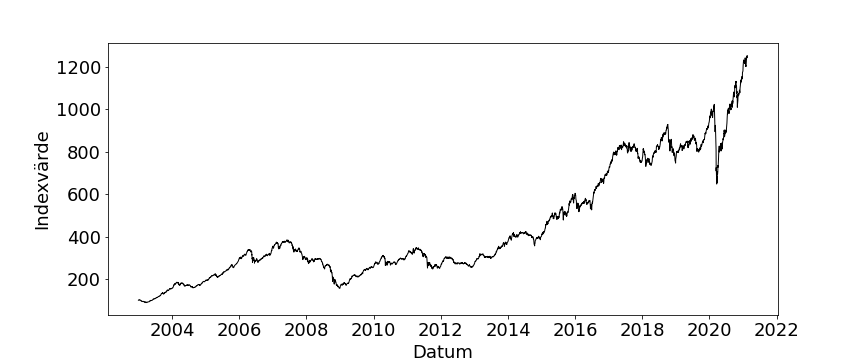
\includegraphics[width=\linewidth]{index.png}
\centering
\end{figure}


\begin{table}[H]
\caption{Deskprivtiv statistik över stängningspriser för OMXSSC mellan 1 januari 2003 och 14 februari 2021}
\resizebox{\columnwidth}{!}{
\begin{tabular}{@{}llllllllll@{}}
\cmidrule(r){1-8}
%
Index  & Start      & Slut       & N    & Min.    & Medelvärde & Max.     & SD  \\ \cmidrule(r){1-8}
OMXSSC & 2003-01-01 & 2021-02-14 & 4564 & 88,54 & 436,45   & 1254,09 & 264,05  \\ \cmidrule(r){1-8}
\end{tabular}}
\end{table}

I Figur 4.2 syns den logaritmerade avkastningsserien där perioder med hög volatilitet kännetecknas av aggressiva prisförändringar. I Tabell 4.2 visas sedan deskriptiv statistik. 

\begin{figure}[H]
\caption{Logaritmerad avkastningsserie för OMXSSC mellan 1 januari 2003 och 14 februari 2021}
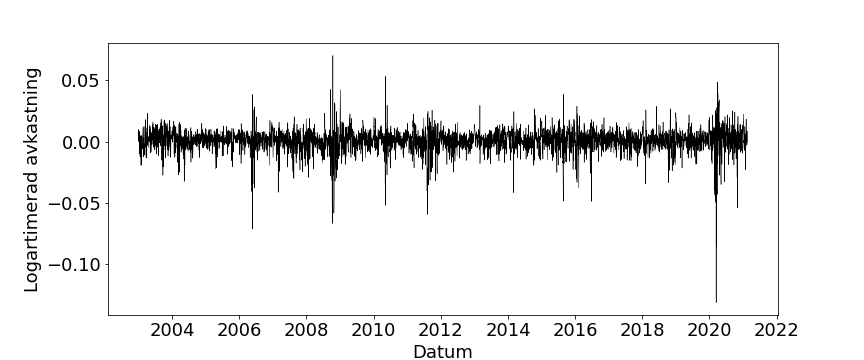
\includegraphics[width=\linewidth]{logreturns.png}
\centering
\end{figure}


\begin{table}[H]
\caption{Deskriptiv statistik över logaritmerad avkastning för OMXSSC mellan 1 januari 2003 och 14 februari 2021}
\begin{tabular}{@{}llllllllll@{}}
\cmidrule(r){1-7}
%
Index  & Min.    & Medelvärde & Max    & SD     & Skrevhet & Kurtosis \\ \cmidrule(r){1-7}
OMXSSC & -0,0875 & 0,0056     & 0,0701 & 0,0006 & -1,4438  & 12,9149  \\ \cmidrule(r){1-7}
\end{tabular}
\end{table}

Eftersom logaritmerade priser är svårtolkade transformeras dessa om till prisnivå efter att modellen gjort sina skattningar. Låt $\hat{\theta_t}$ vara predicerad logaritmerad avkastning för tidpunkt $t$ och $\phi$ är träningsperiodens sista prisdatapunkt. Då kan den kumulativa summan av den logaritmerade avkastningen exponentieras för att få prisnivån enligt

\begin{equation}
    \text{Prisnivå} =  exp\Big({\sum\limits_{t=1}^n \hat{\theta_{t}}} + ln(\phi)\Big)
\end{equation}

Prediktioner görs $t=\{1, 3, 5, 21, 63\}$ dagar fram i tiden, där $t=1$ motsvarar en börsdag,  $t=3$ en halv börsvecka, $t=5$ en hel börsvecka, $t=21$ en börsmånad och $t=63$ ett börskvartal. Vidare delas 75 procent av datamaterialet in i träningsdata som sträcker sig från 1 januari 2003 till 31 juli 2016. Resterande del av datamaterialet utgörs av testdata och sträcker sig mellan den 3 augusti 2016 till den 14 febuari 2021. 

\newpage
%%%%%%%%%%%%%% RESULTAT %%%%%%%%%%%%%%%
\section{Resultat}
\subsection{ARMA-GARCH modellvalidering}
För att testa om tidsserien är stationär används ett augmented Dickey-Fuller-test som är signifikant med $p<0,01$ och optimalt antal laggar är 1 (se bilaga C). Vidare förkastas nollhypotesen om att tidsserien inte är stationär, således behövs ingen differentiering i ARIMA, dvs. en ARIMA(p,0,q)=ARMA(p,q) är tillräcklig. För att validera om feltermen behöver modelleras med GARCH eller om det räcker med en ARIMA väljs den optimala ARIMA-modellen utifrån datan med funktionen \textit{auto.arima} i R. Valet görs baserat på AIC. Detta ger en ARIMA(1,0,1) som sammanställs i Tabell 5.1. För att säkerställa oberoende i feltermerna görs ett Ljung-Box test. Det visar att residualerna i ARIMA-modellen inte är beroende (se bilaga D). Slutligen testas efter heteroskedasticitet i ARIMA-modellen med LM-test. Nollhypotesen förkastas, $p=0.00$, och alltså finns tydliga tecken på heteroskedasticitet (se bilaga E). Detta indikerar att feltermen egentligen bör modelleras med GARCH. 

\begin{table}[H]
\caption{Sammanfattning av ARIMA(1,0,1)-modellen}
\begin{tabularx}{\textwidth}{c *{6}{Y}}
\toprule

Parameter  & Skattning & Standardfel & p-värde \\
\hline

$\delta$        & 0,0005  & 0,0002  & $0,0087$   \\
$\phi_1$        & 0,6737  & 0,0670  & $<2,2\cdot10^{-16}$   \\

$\theta_1$      & -0,5574 & 0,0754  &  $1,4\cdot10^{-13}$   \\
\midrule

Informationskriterier  & &  &  \\
\hline

Log likelihood        & 11.358,46 \\
AIC                   & -22.708,91 \\

BIC                   & -22.683,36 \\
\bottomrule
\end{tabularx}
\footnotesize{Notera att samtliga parametrar är signifikant skilda från 0 på 5 procent nivå.}
\end{table}

Eftersom det finns tecken på heteroskedasticitet och ingen differentiering behövs appliceras ARMA-GARCH. AIC och BIC visar att ARMA(1,1)-GARCH(1,1) är den bästa möjliga modellen (se bilaga G för alla modeller som utvärderas). Ett Ljung-Box test görs även för denna modell, för att vara säker på att residualerna är oberoende. Även det är insignifikant, $p=0.5033$ (se Bilaga D). Nedan följer en sammanställning över modellen och i bilaga F illustreras prediktioner baserat på modellen, inklusive konfidentsintervall.

\begin{table}[H]
\caption{Sammanfattning av ARMA(1,1)-GARCH(1,1)-modellen}
\begin{tabularx}{\textwidth}{c *{6}{Y}}
\toprule
Parameter  & Skattning & Standardfel & p-värde \\
\hline

$\delta$      & 0,0002         & $6,1\cdot10^{-5}$ & 0,0012           \\
$\phi_1$      & 0,7707         & 0,0492         & $<\cdot10^{-16}$    \\

$\theta_1$    & -0,6484        & 0,0593         & $<2\cdot10^{-16}$    \\
$w$           & $4,16*10^{-6}$ & $5,66*10^{-7}$ & $1,89\cdot10^{-13}$  \\

$\alpha_1$    & 0,1716         & 0,0154         & $<2\cdot10^{-16}$    \\
$\beta_1$     & 0,7721         & 0,0180         & $<2\cdot10^{-16}$    \\ 
\midrule

Informationskriterier  & &  &  \\
\hline

Log likelihood & 11.926,87       &                &                  \\
AIC            & -6,9652        &                &                   \\

BIC            & -6,9544         &                &                   \\
\bottomrule
\end{tabularx}
\footnotesize{Notera att samtliga parametrar är signifikant skilda från 0 på 5 procent nivå.}
\end{table}






$\delta, \phi_1$ och $\theta_1$ förekommer även i ARIMA-modellen. Som synes är de annorlunda i ARMA-GARCH. Detta beror på modelleringen av feltermen i GARCH-komponenten ändrar parameterskattningarna.

\subsection{RMSE och MAPE}
I Tabell 5.3 sammanfattas resultaten av RMSE och MAPE för LSTM och ARMA-GARCH vid den enskilda skattningen.

\begin{table}[H]
\caption{RMSE \& MAPE vid en enskilda skattningar}
\begin{tabularx}{\textwidth}{c *{6}{Y}}
\toprule


 & \multicolumn{2}{c}{LSTM}  
 & \multicolumn{2}{c}{ARMA-GARCH}\\

\cmidrule(lr){2-3} \cmidrule(l){4-5}
$t ^\dagger$  & \emph{RMSE} & \emph{MAPE(\%)} & \emph{RMSE} & \emph{MAPE(\%)} \\

\midrule

1  &  1,18    &  0,19   &   0,02  & 0,00 \\
3  &  4,05    & 0,51    &  7,52   & 0,71 \\

5  &  4,32    & 0,39    &  9,85   & 0,71 \\
21 &  20,97   &  0,89   &  2,32   & 0,54 \\

63 &  150,21  & 2,93    &  43,55  & 1,06 \\

\bottomrule
\end{tabularx}
\footnotesize{$^\dagger$ Antal börsdagar som prediceras}
\end{table}






Utifrån tabellen syns att LSTM har lägre prediktionsfel än ARMA-GARCH på 3- och 5 dagars sikt medan ARMA-GARCH överträffar LSTM på 1-, 21- och 63 dagars sikt.

RMSE och MAPE korsvalideras även över 1.000 perioder. Medelvärden av måtten presenteras nedan. 




\begin{table}[H]
\caption{Genomsnittligt RMSE \& MAPE över 1.000 skattningar}
\begin{tabularx}{\textwidth}{c *{6}{Y}}
\toprule

 & \multicolumn{2}{c}{LSTM} 
 & \multicolumn{2}{c}{ARMA-GARCH}\\

\cmidrule(lr){2-3} \cmidrule(l){4-5}
$t ^\dagger$  & \emph{RMSE} & \emph{MAPE(\%)} & \emph{RMSE} & \emph{MAPE(\%)} \\

\midrule

1  & 4,97    &  0,61   & 4,91    & 0,61 \\
3  &  12,16  & 0,91    &  11,90  & 0,91 \\

5  &  19,82  & 1,19    &  19,18  &  1,16 \\
21 & 92,26   &  2,75   & 85,88   & 2,57 \\

63 &  322,02 & 5,40    &  294,07 & 5,02 \\

\bottomrule
\end{tabularx}
\footnotesize{$^\dagger$ Antal börsdagar som prediceras}
\end{table}

Ingen av måtten är i signifikant bättre än det andra i någon av de utforskade perioderna.

\subsection{Precision, Känslighet och F-värde}
Nedan ges en sammanfattning över känsligheten, precisionen och F-värdet för de bägge modellerna för varje period vid en enskild skattning.

\begin{table}[H]
\caption{Precision, känslighet och F-värde vid en enskild skattning}

\begin{tabularx}{\textwidth}{c *{6}{Y}}
\toprule

 & \multicolumn{2}{c}{Precision}  
 & \multicolumn{2}{c}{Känslighet}  
 & \multicolumn{2}{c}{F-värde}\\

\cmidrule(lr){2-3} \cmidrule(l){4-5} \cmidrule(l){6-7}
$t ^\dagger$  & \emph{LSTM} & \emph{ARMA-GARCH} & \emph{LSTM} & \emph{ARMA-GARCH} & \emph{LSTM} & \emph{ARMA-GARCH} \\

\midrule

1  & 1       &  1      & 1    & 1   & 1       & 1      \\
3  & 0,33    &  0,33   &  1   & 1   & 0,50    & 0,50   \\

5  & 0,20    &  0,20    &  1   & 1   & 0,33    & 0,33   \\
21 & 0,81    &  0,81  & 1  & 1   & 0,89    & 0,89   \\

63 & 0,94    &  0,94   &  1  & 1   & 0,97   & 0,97    \\

\bottomrule
\end{tabularx}
\footnotesize{$^\dagger$ Antal börsdagar som prediceras}
\end{table}

Modellerna ger identiska resultat. Att känsligheten är 1 för bägge modellerna beror på att de identifierar en stigande prisnivå, därav blir andelen stigande prediktioner som är korrekta hög (se bilaga F). LSTM har en nedgång vid ungefär 30 perioder samtidigt som index uppvisar en negativ utveckling, vilket förklarar varför känsligheten inte påverkas av den nedåtgående prisnivån.

För att säkerställa att resultaten ovan inte enbart är en effekt av den valda tidpunkten görs korsvalidering över 1.000 skattningar. I Tabell 5.6 sammanfattas resultaten.

\begin{table}[H]
\caption{Genomsnittliga precision, känslighet och F-värde över 1.000 skattningar}

\begin{tabularx}{\textwidth}{c *{6}{Y}}
\toprule

 & \multicolumn{2}{c}{Precision}  
 & \multicolumn{2}{c}{Känslighet}  
 & \multicolumn{2}{c}{F-värde}\\

\cmidrule(lr){2-3} \cmidrule(l){4-5} \cmidrule(l){6-7}
$t^\dagger$  & \emph{LSTM} & \emph{ARMA-GARCH} & \emph{LSTM} & \emph{ARMA-GARCH} & \emph{LSTM} & \emph{ARMA-GARCH}  \\

\midrule

1  & 0,01    &  0,08*   & 0,01    & 0,08*  & 0,01    & 0,08*       \\
3  & 0,17    &  0,28*      &  0,28   & 0,37*   & 0,20    & 0,29*     \\

5  & 0,23   &  0,36*      &  0,33   &  0,45*  & 0,25   & 0,37*     \\
21 & 0,31    &  0,61*    & 0,37    & 0,72*   & 0,31    & 0,61*     \\

63 & 0,37   & 0,66*      &  0,33  & 0,86*     & 0,29   & 0,70*    \\

\bottomrule
\end{tabularx}
\footnotesize{* $p<0.05$ medelvärdestest med alternativhypotesen att ARMA-GARCH är högre än LSTM} \\
\footnotesize{$^\dagger$ Antal börsdagar som prediceras}
\end{table}

ARMA-GARCH är i snitt bättre gällande samtliga mått oavsett hur långa prediktioner som görs. Att värdena på precision och känslighet är identiska vid en periods prediktion beror på att testen testar samma sak då. Antingen är det en sann stigande och då ger bägge måtten 1 eller är det inte sant stigande och då returnerar båda måtten 0 (se ekvation 3.17 och 3.18).


\subsection{Utvärdering av handelsstrategi}
För utvärdering av handelsstrategin jämförs hur stor procentuell avkastning modellerna genererat under varje givet tidsintervall. I Tabell 5.7 presenteras den procentuella avkastningen av att handla med respektive strategi samt hur många ordrar algoritmen gör under de 1.000 perioderna. För att kunna utvärdera strategierna används den passiva investeringsstrategin som riktmärke - en strategi som genererat 61,9 procent avkastning över perioden.

\begin{table}[H]
\caption{Avkastning efter handel över 1.000 perioder$^\ddagger$}
\begin{tabularx}{\textwidth}{c *{6}{Y}}
\toprule

 & \multicolumn{2}{c}{LSTM}
 & \multicolumn{2}{c}{ARMA-GARCH}\\

\cmidrule(lr){2-3} \cmidrule(l){4-5}
$t^\dagger$  & \emph{Avkastning(\%)} & \emph{Antal ordrar} & \emph{Avkastning(\%)} & \emph{Antal ordrar} \\

\midrule

1  &  12,53    &  51   & 117,9    & 78 \\
3  &  -0,42   & 87    &  117,05 & 62 \\

5  &  7,69   & 121   &  112,64  &  54 \\
21 & 8,26    &  137   & 92,27   & 5 \\

63 &  8,26   & 188   &  59,20 & 2 \\

\bottomrule
\end{tabularx}
\footnotesize{$^\ddagger$ Under perioden 2016-08-03 - 2020-07-25. En passiv strategi genererade en totalavkastning på 61,90 procent under samma period.}\\
\footnotesize{$^\dagger$ Antal börsdagar som prediceras}
\end{table}


Ur tabellen går det att utröna att LSTM presterar sämre än den passiva strategin oavsett vilken tidsperiod prediktionerna baseras på. ARMA-GARCH presterar bättre än den passiva strategin på en till 21 perioders sikt och sämre därefter. 

\newpage
\section{Diskussion}
Denna studie ämnade att undersöka om en djupinlärningsmodell med fördel kan användas istället för en ekonometrisk modell på svenskt börsindex. Därutöver undersöktes om en algoritmisk handelsstrategi som är bättre än indexet kan byggas. För att besvara dessa användes de tre olika valideringstyperna:

\begin{itemize}
\item Prediktionsfel (MAPE och RMSE)
\item Binär klassificering (F-värde, precision och känslighet)
\item Simulerad handel (Procentuell avkastning)
\end{itemize}

Resultatet utvärderades först vid en enskild skattning. De resultaten gjorde det dock svårt att avgöra om skillnaderna var permanenta eller enbart en konsekvens av den punkt på tidsserien där prediktionerna gjordes, vilket var varför korsvalidering över 1.000 skattningar applicerades. Därför läggs större delen i diskussionen åt att diskutera denna.

Rörande prediktionsfel, mätt med RMSE och MAPE, visade analysen att ingen av modellerna var signifikant bättre än den andra oavsett hur många perioder fram i tiden som predicerades. Föga förvånande var kortare prediktioner mer precisa än långa. 

Den binära klassificeringen av pris upp- och nedgångar utgjordes av känslighet, precision och F-värde. Oavsett vilket av måtten som används eller hur långa prediktioner som görs presterar ARMA-GARCH i genomsnitt bättre. Väl värt att notera är att LSTM inte är bättre än att slumpmässigt gissa (50 procent rätt) avseende precision eller känslighet. På 1, 3 och 5 dagars sikt är inte ARMA-GARCH heller det, men på 21 och 63 perioders sikt ger ARMA-GARCH mer än 50 procent rätt på både precision och känslighet. Detta visar på att även om genomsnittligt RMSE och MAPE är högt på längre perioder så är modellen åtminstone bra på att identifiera en framtida stigande prisnivå. Intressant är också att samtliga modeller blir bättre vid längre prediktioner, vilket är rakt motsatt resultatet av prediktionsfel. Detta kan tänkas bero på att marknaden under längre perioder uppvisar en positiv prisutveckling, vilket inte gäller i samma utsträckning på kort sikt (se Figur 4.1), det räcker alltså för modellerna att identifiera en stigande trend för att ha rätt.   

Resultaten av simulerad handling över 1.000 perioder visade entydigt att ARMA-GARCH var att föredra oavsett hur långt in i framtiden det prediceras. Det var även tydligt, och föga förvånande, att kortsiktiga prediktioner gav högre avkastning än långsiktiga. ARMA-GARCH överträffade även den passiva strategin upp till 21 perioders prediktion medan LSTM underpresterade samma strategi oavsett prediktionsperiod. Som tidigare diskuterats kan den passiva strategin liknas vid en slumpvandring och givet att EMH rådde ska det därför inte ha gått att finna en modell som var bättre än den denna. Men eftersom ARMA-GARCH visade sig generera högre avkastning än den passiva strategin kan EMH förkastas under den studerade perioden. En ARMA-GARCH kan användas för att applicera en algoritmisk handelsstrategi som presterar bättre än index under den studerade perioden.

Intressant är att modellerna var oskiljbara rörande prediktionsfel men skillnaden i avkastning var stor. Ur ett bredare perspektiv kan dessa resultat tänkas påvisa att en modell som presterar väl på modellvalideringen inte nödvändigtvis är samma modell som genererar högst avkastning. Det belyser vikten av att inte enbart basera modellval på lägsta möjliga prediktionsfel. 

Tabell 6.1 illustrerar samtliga slutsatser som nås i diskussionen ovan.

\begin{table}[H]
\caption{Sammanfattning av jämförelsen mellan modellerna på de tre valideringstyperna}

\begin{tabularx}{\textwidth}{c *{6}{Y}}
\toprule
$t ^\dagger$  & Prediktionsfel & Exakthet & Avkastning \\
\hline

1      & Oskiljbara          & ARMA-GARCH                 & ARMA-GARCH          \\
3      & Oskiljbara          & ARMA-GARCH          & ARMA-GARCH    \\

5      & Oskiljbara          & ARMA-GARCH         &ARMA-GARCH   \\

21     &  Oskiljbara         & ARMA-GARCH         & ARMA-GARCH   \\


63     & Oskiljbara         & ARMA-GARCH         & ARMA-GARCH    \\ 

\bottomrule
\end{tabularx}
\footnotesize{$^\dagger$ Antal börsdagar som prediceras}
\end{table}

När resultatet sätts i förhållande till tidigare studier nås flera intressanta insikter. Flera tidigare studier nådde slutsatsen att LSTM var åtminstone lika bra och ofta bättre än ARIMA. Att denna studie visat andra resultat kan tänkas bero på tre faktorer. För det första har flera av studierna applicerat ARIMA utan GARCH-komponent. Som diskuterades och även påvisades är antagandet om homoskedasticitet sällan uppfyllt i finansiella tidsserier. ARIMA utan GARCH-komponent är således suboptimalt. En andra faktor som kan ha påverkat var specifikationen av LSTM. Modellen använde en lagg eftersom det var jämförbart med ARMA-GARCH. Fler laggar hade i teorin kunnat ge ett annat resultat. Dock ökar risken för en överanpassning av data markant -  modellen anpassas för nära till den befintliga datan vilket hämmar förmågan att förutspå utanför urvalet. I denna studie valdes alltså antal laggar baserat på teori snarare än empiri, vilket minskar risken för överanpassning men kan ha gjort förutsättningar för LSTM mindre fördelaktiga. Den tredje faktorn är att det i denna studie har säkerställts att samtliga antaganden kring ARMA-GARCH är uppfyllda. Som Paliwal och Kumar \parencite*{paliwal2009neural} visat har det i tidigare jämförelser mellan statistiska modeller och neurala nätverk ofta slarvats med antaganden. 

Ur ett användarvänlighetsperspektiv är ARMA-GARCH att föredra. LSTM är svårtolkad och som påpekades i metoden finns det begränsat med forskning kring hur den ska specifieras. LSTM är icke-parametrisk och det går således inte heller att dra slutsatser kring parametrars signifikansnivåer. En fördel med LSTM är dock att den är enkel att applicera eftersom den bara har ett antagande att uppfylla. 

\subsection{Felkällor}
Enligt Hyndman och Athanasopoulos \parencite*[][,s.452 f.]{hyndman2018forecasting} finns flera felkällor till alla tidsseriemodeller. Den slumpmässiga feltermen, benämnd \(e_t\), är såklart en av dem. Utöver den finns åtminstone tre ytterligare felkällor. 

Den första är estimaten av parametrar i modellerna i såväl ARMA-GARCH som LSTM. En viss osäkerhet kommer från att modellerna är baserade på ett stickprov, parametrarna är optimala utifrån stickprovet och inte nödvändigtvis utifrån populationen. Utöver det har denna studie valt ARMA-GARCH-modell baserat på AIC och BIC, men andra liknande mått för utvärdering finns som hade kunnat ge annorlunda resultat. Hannan-Quinn Information Criterion (HQC) är ett sådant \parencite{hannan1979determination}. På samma vis hade LSTM-modellen kunnat specifieras annorlunda, med viss försiktighet rörande överanpassning hade de använda parametrarna kunnat optimerats mer till datasetet och gett andra estimat.

Den andra är valet av modell. En modell kommer alltid vara en förenkling av verkligheten, vilket i sig leder till fel, men olika modeller kan ge mer eller mindre fel. Exempelvis används andra typer av GARCH-modeller inom finansiell analys, såsom exponentiell GARCH (EGARCH) \parencite{nelson1991conditional}. Vidare hade ARMA-komponenten kunnat bytas ut mot ARFIMA (Autoregressive Fractionally Integrated Moving Average), som visat sig effektiv när tidsserier behöver ha ett långt minne, precis som LSTM \parencite{taqqu1995estimators}. Angående LSTM hade det varit möjligt att använda en simplare modell. Neurala nätverk, som LSTM är en underkategori till, används frekvent inom området \parencite[se t.ex.][]{rather2015recurrent}. Det finns även andra typer av LSTM, såsom "Deep LSTM" med flera lager av neuroner \parencite[se applikation i][]{hansson2017stock}. Därutöver baserades valet av modell i samtliga perioder av korsvalideringen på vilken modell som var bäst vid sista träningsperioden. Andra resultat hade möjligen kunnat nås om modellen vid varje enskild tidpunkt modellerades om och parametrarna optimerades utifrån den nya datapunkten som tillförts. Det är inte heller säkert att alla modellantaganden uppfylls i alla 1.000 perioder, vilket kan påverkat ARMA-GARCH prestation. 

Slutligen gäller inte nödvändigtvis förutsättningarna som var när datan insamlades i framtiden. Ett exempel på denna felkälla är Bitcoin. I maj 2016 var en Bitcoin värd ca. 450 USD. När denna uppsats skriv i maj 2021 är en Bitcoin värd ca. 64.000 USD. En ökning med över 14.000 procent \parencite{yahoo_bitcoin}. Det förefaller osannolikt att en modell som var bra innan ökningen fortfarande håller måttet. Poängen är alltså att framtida applikationer av de modeller som använts i denna studie inte nödvändigtvis genererar samma resultat.

\newpage
%%%%%%%%%%%%%%%%%%
% SLUTSATS %%%%%%%%%%%%%%%%%%%
\section{Slutsats}
Denna studie ämnade att besvara frågorna \emph{"Kan en djupinlärningsmodell med fördel användas som substitut för en ekonometrisk modell på svenskt börsindex?"} samt \emph{"Kan en algoritmisk handelsstrategi som ger högre avkastning än utvecklingen hos ett svenskt småbolagsindex skapas?"}. Resultatet till den första frågan visade att om minimering av prediktionsfel är målet är modellerna lika kapabla. Om målet snarare är exakthet är ARMA-GARCH att föredra, likaså om målet är generera högsta möjliga avkastning. ARMA-GARCH kan även användas för att bygga en handelsstrategi som är bättre än ett svenskt småbolagsindex utveckling.

Vidare studier kan med fördel undersöka om resultaten håller för andra index än OMXSSC. Detta vore intressant eftersom slutsatserna av denna studie delvis går emot tidigare forskning. Som diskuterades i felkällor kan framtida studier även djupdyka i olika varianter av ARMA-GARCH (såsom ARFIMA-EGARCH) respektive LSTM (såsom Deep LSTM).



%%%%%%%%%%%%%%%%%%% Referenser %%%%%%%%%%%%%%%%%%%
\newpage
\section*{Referenser}
\addcontentsline{toc}{section}{Referenser}
\printbibliography[heading=none]




%%%%%%%%%%%%%%%%%%% BILAGOR %%%%%%%%%%%%%%%%%%%
\newpage

\appendix
\section*{Bilagor}
\addcontentsline{toc}{section}{Bilagor}
\renewcommand{\thesubsection}{\Alph{subsection}}

\subsection{Python- och R-paket}
Följande paket användes i Python version 3.8 respektive R version 4.0 för att skapa modellerna. 

\textbf{R} \par
\textit{forecast} användes för att skapa ARIMA-modellen. \par
\textit{aTSA} användes för att testa för heteroskedasticitet. \par
\textit{fGarch} användes för att skapa ARMA-GARCH-modellen. \par
\textit{urca} användes för ADF-Fuller-testet. \par
\textit{stats} användes bl.a. för Ljung-Box test. \par

\textbf{Python} \par
\textit{Scikit-learn} och \textit{Keras} användes för att skapa LSTM-modellen.

\subsection{Indexbeståndsdelar 12 februari 2021}
\begin{table}[H]
\scalebox{0.75}{
\begin{tabular}{|l|l|l|l|}
\hline
Namn & Kortnamn & Namn & Kortnman \\ \hline
\rowcolor[HTML]{EFEFEF} 
Abliva AB & ABLI & Magnolia Bostad AB & MAGNO \\ \hline
Actic Group AB & ATIC & Maha Energy AB & MAHAa \\ \hline
\rowcolor[HTML]{EFEFEF} 
Active Biotech AB (publ) & ACTI & Malmbergs Elektriska AB (publ) & MEABb \\ \hline
Alligator Bioscience AB & ATORX & Medivir AB & MVIRb \\ \hline
\rowcolor[HTML]{EFEFEF} 
Anoto Group AB & ANOT & Micro Systemation AB (publ) & MSABb \\ \hline
Arctic Paper SA & ARP & Midway Holding AB & MIDWb \\ \hline
\rowcolor[HTML]{EFEFEF} 
Arise AB & ARISE & Midway Holding AB & MIDWa \\ \hline
Ascelia Pharma AB & ACELP & Moberg Pharma AB (publ) & MBPH \\ \hline
\rowcolor[HTML]{EFEFEF} 
Atvexa AB & ATVEXAb & Moment Group AB & MOMENT \\ \hline
B3 Consulting Group AB (publ) & B3 & MultiQ International AB & MULQ \\ \hline
\rowcolor[HTML]{EFEFEF} 
BE Group AB (publ) & BEGR & Nelly Group AB (publ) & NELLY \\ \hline
Beijer Electronics Group AB & BELE & Net Insight AB & NETIb \\ \hline
\rowcolor[HTML]{EFEFEF} 
Bergs Timber AB (publ) & BRGb & NGS Group AB & NGSG \\ \hline
BioInvent International AB & BINV & Nilorngruppen AB & NILb \\ \hline
\rowcolor[HTML]{EFEFEF} 
Bjorn Borg AB & BORG & Note AB (publ) & NOTE \\ \hline
Bong AB & BOLJ & Novotek AB & NTEKb \\ \hline
\rowcolor[HTML]{EFEFEF} 
Boule Diagnostics AB & BOUL & Odd Molly International AB & ODD \\ \hline
C Rad AB & CRADb & Ortivus AB & ORTIb \\ \hline
\rowcolor[HTML]{EFEFEF} 
Christian Berner Tech Trade AB & CBTTb & Ortivus AB & ORTIa \\ \hline
Concejo AB (publ) & CNCJOb & Oscar Properties Holding AB & OP \\ \hline
\rowcolor[HTML]{EFEFEF} 
Concordia Maritime AB & CCORb & Poolia AB & POOLb \\ \hline
Dedicare AB (publ) & DEDIC & Precise Biometrics AB & PREC \\ \hline
\rowcolor[HTML]{EFEFEF} 
Doro AB & DORO & Prevas AB & PREVb \\ \hline
Duroc AB & DURCb & Profilgruppen AB & PROFb \\ \hline
\rowcolor[HTML]{EFEFEF} 
Egetis Therapeutics AB (publ) & EGTX & Projektengagemang Sweden AB & PENGb \\ \hline
Electra Gruppen AB (publ) & ELEC & Qliro AB & QLIRO \\ \hline
\rowcolor[HTML]{EFEFEF} 
Elos Medtech AB & ELOSSb & Railcare Group AB & RAILG \\ \hline
Empir Group AB & EMPIRb & Rnb Retail and Brands AB (publ) & RNBS \\ \hline
\rowcolor[HTML]{EFEFEF} 
Endomines AB (publ) & ENDO & Saniona AB & SANION \\ \hline
Eniro AB & ENRO & Semcon AB & SEMC \\ \hline
\rowcolor[HTML]{EFEFEF} 
Episurf Medical AB & EPISb & Sensys Gatso Group AB & SENS \\ \hline
Etrion Corp & ETRN & SERNEKE Group AB (publ) & SRNKEb \\ \hline
\rowcolor[HTML]{EFEFEF} 
Ework Group AB & EWRK & SinterCast AB & SINT \\ \hline
Feelgood Svenska AB (publ) & FEEL & Softronic AB & SOFb \\ \hline
\rowcolor[HTML]{EFEFEF} 
FM Mattsson Mora Group AB & FMMb & Starbreeze AB & STZEb \\ \hline
FormPipe Software AB & FPIP & Starbreeze AB & STZEa \\ \hline
\rowcolor[HTML]{EFEFEF} 
Gaming Innovation Group Inc & GIGSEK & Stockwik Forvaltning AB & STWK \\ \hline
GHP Specialty Care AB & GHP & Strax AB & STRAX \\ \hline
\rowcolor[HTML]{EFEFEF} 
Green Landscaping Group AB & GREENL & Studsvik AB & SVIK \\ \hline
Hanza Holding AB & HANZA & Svedbergs i Dalstorp AB & SVEDb \\ \hline
\rowcolor[HTML]{EFEFEF} 
Image Systems AB & ISY & TradeDoubler AB & TRAD \\ \hline
Immunicum AB & IMMUN & Vicore Pharma Holding AB & VICOR \\ \hline
\rowcolor[HTML]{EFEFEF} 
Irras AB & IRRAS & Viking Supply Ships AB & VSSABb \\ \hline
Josemaria Resources Inc & JOSE & Wise Group AB & WISE \\ \hline
\rowcolor[HTML]{EFEFEF} 
KABE Group AB & KABEb & Xbrane Biopharma AB & XBRANE \\ \hline
Karolinska Development AB & KDEV & ZetaDisplay AB & ZETA \\ \hline
\rowcolor[HTML]{EFEFEF} 
Lammhults Design Group AB & LAMMb & \multicolumn{2}{l|}{\cellcolor[HTML]{EFEFEF}} \\ \hline
\end{tabular}}
\end{table}

\subsection{ADF-test}

\begin{table}[H]
\caption{Augmented Dickey-Fuller Test för stationäritet}
\begin{tabularx}{\textwidth}{c *{4}{Y}}
\multicolumn{3}{l}{Optimalt antal laggar: 1 (valt med AIC)} \\
\multicolumn{3}{l}{H0: Ingen stationäritet, H1: Stationäritet} \\
\toprule
  & Skattning & Standardfel & p-värde \\
\midrule
ADF teststatistika  &  -0.791    &  0.022 & $< 2\cdot10^{-16}$  \\
\bottomrule
\end{tabularx}
\end{table}

\vspace{0.5cm}
\subsection{Residualanalys}

\begin{table}[H]
\caption{Ljung-Box test för ARIMA(1,0,1)}
\begin{tabularx}{\linewidth}{c *{3}{Y}}
\multicolumn{3}{l}{H0: Oberoende residualer, H1: Ej oberoende residualer} \\
\toprule
$\chi^2$ & Frihetsgrader & p-värde \\
\midrule
0.16409  &  1    &  0.6854  \\
\bottomrule
\end{tabularx}
\end{table}

\begin{table}[H]
\caption{Ljung-Box test för ARMA(1,1)-GARCH(1,1)}
\begin{tabularx}{\linewidth}{c *{3}{Y}}
\multicolumn{3}{l}{H0: Oberoende residualer, H1: Ej oberoende residualer} \\
\toprule
$\chi^2$ & Frihetsgrader & p-värde \\
\midrule
0.4484  &  1    &  0.5031  \\
\bottomrule
\end{tabularx}
\end{table}

\begin{figure}[H]
\caption{Fördelning av ARMA(1,1)-GARCH(1,1) residualer}
\includegraphics[width=1\linewidth]{histogram-residuals.png}
\centering
\end{figure}

\vspace{0.5cm}
\subsection{LM-test}

\begin{table}[H]
\caption{Lagrange-Multiplier test}
\begin{tabularx}{\linewidth}{c *{3}{Y}}
\multicolumn{3}{l}{H0: Homoskedasticitet, H1: Heteroskedasticitet} \\
\toprule
Order & LM & p-värde \\
\midrule
4  &  2248    &  0  \\
8  &  1059    &  0  \\
12  &  657    &  0  \\
16  &  482    &  0  \\
20  &  378    &  0  \\
24  &  312    &  0  \\
\bottomrule
\end{tabularx}
\end{table}

\subsection{Prediktioner vid t=1}
\begin{figure}[H]
\caption{LSTM-prediktioner vid enskild tidpunkt}
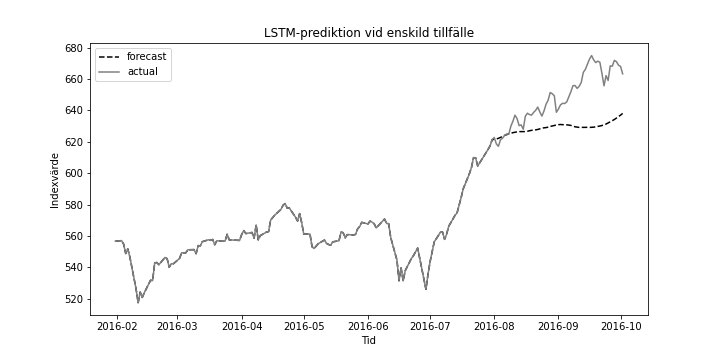
\includegraphics[width=\linewidth]{lstm_pred.png}
\centering
\end{figure}
Notera att LSTM inte har konfidensintervall.

\begin{figure}[H]
\caption{ARMA-GARCH-prediktioner vid enskild tidpunkt}
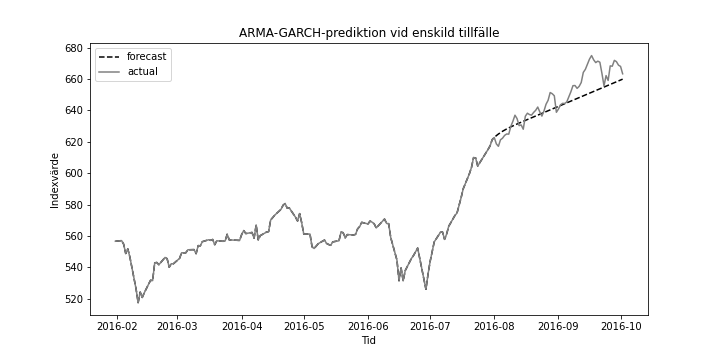
\includegraphics[width=\linewidth]{arma_garch_pred.png}
\centering
\end{figure}

\begin{figure}[H]
\caption{ARMA-GARCH-prediktioner 5 perioder fram vid enskild tidpunkt med prediktionsintervall}
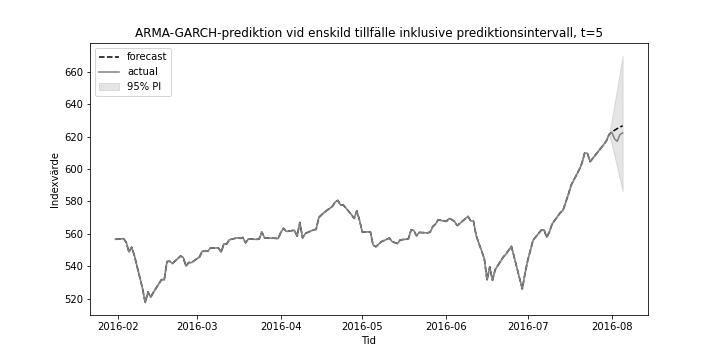
\includegraphics[width=\linewidth]{arma_garch_pred_interval_5.png}
\centering
\end{figure}

\begin{figure}[H]
\caption{ARMA-GARCH-prediktioner 63 perioder fram vid enskild tidpunkt med prediktionsintervall}
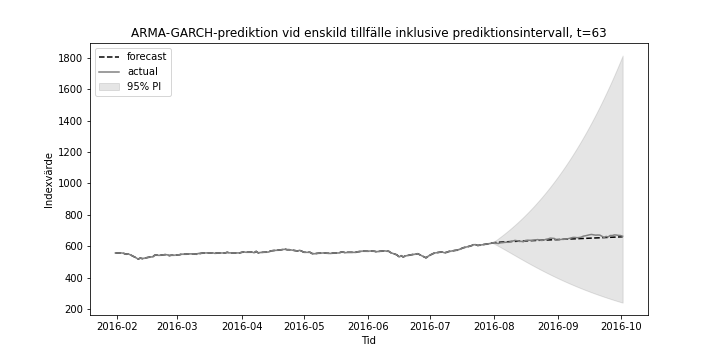
\includegraphics[width=\linewidth]{arma_garch_pred_interval_63.png}
\centering
\end{figure}
Notera hur prediktionsintervallen ska 63 perioder framåt är enorma jämfört med 5 perioder framåt. Detta beror såklart på enormt stora osäkerheter vid så långa prediktioner.

\subsection{AIC och BIC för ett urval av modeller}
Ju lägre värde, desto bättre. ARMA(1,1)-GARCH(1,1) ger lägst resultat.

\begin{table}[H]
\caption{Specifikationer för ARMA-GARCH: AIC \& BIC}
\begin{tabularx}{\textwidth}{c *{6}{Y}}
\toprule
Modell  & AIC & BIC  \\
\hline

ARMA(0,0)-GARCH(1,0)            & -6,782                &   -6,777     \\

ARMA(0,0)-GARCH(1,1)            & -6,938         & -6,931    \\


ARMA(0,1)-GARCH(1,1)            & -6,951         & -6,942   \\

ARMA(1,0)-GARCH(1,1)           & -6,954         & -6,944   \\


\textbf{ARMA(1,1)-GARCH(1,1)}           & \textbf{-6,965}          & \textbf{-6,954}
    \\ 

ARMA(1,1)-GARCH(2,1)           & -6,965         & -6,952   \\ 

ARMA(1,1)-GARCH(2,2)           & -6,964        & -6,950
   \\ 

ARMA(2,1)-GARCH(2,2)           &-6,964        & -6,948    \\ 

ARMA(2,2)-GARCH(2,2)           & -6,963         &  -6,946
   \\ 

\bottomrule
\end{tabularx}
\end{table}

\vspace{0.5cm}
\subsection{Histogram över logaritmerad avkastning med KDE}
\begin{figure}[H]
\caption{Histogram logaritmerad avkastning}
\includegraphics[width=\linewidth]{histogram.png}
\centering
\end{figure}



\end{document}